% Copyright © 2013 Martin Ueding <dev@martin-ueding.de>

% Copyright © 2012-2013 Martin Ueding <dev@martin-ueding.de>

% This is my general purpose LaTeX header file for writing German documents.
% Ideally, you include this using a simple ``% Copyright © 2012-2013 Martin Ueding <dev@martin-ueding.de>

% This is my general purpose LaTeX header file for writing German documents.
% Ideally, you include this using a simple ``% Copyright © 2012-2013 Martin Ueding <dev@martin-ueding.de>

% This is my general purpose LaTeX header file for writing German documents.
% Ideally, you include this using a simple ``\input{header.tex}`` in your main
% document and start with ``\title`` and ``\begin{document}`` afterwards.

% If you need to add additional packages, I recommend not doing this in this
% file, but in your main document. That way, you can just drop in a new
% ``header.tex`` and get all the new commands without having to merge manually.

% Since this file encorporates a CC-BY-SA fragment, this whole files is
% licensed under the CC-BY-SA license.

\documentclass[11pt, ngerman, fleqn, DIV=15, headinclude, BCOR=2cm]{scrartcl}

\usepackage{graphicx}

% Environment to quote the problem. Currently, this is just a new name for the
% quote environment.
\newenvironment{problem}{\begin{quote}\textsf{\textbf{Aufgabenstellung:}}\quad}{\end{quote}}

\setkomafont{caption}{\sf}
\setkomafont{captionlabel}{\usekomafont{caption}}

%%%%%%%%%%%%%%%%%%%%%%%%%%%%%%%%%%%%%%%%%%%%%%%%%%%%%%%%%%%%%%%%%%%%%%%%%%%%%%%
%                                Locale, date                                 %
%%%%%%%%%%%%%%%%%%%%%%%%%%%%%%%%%%%%%%%%%%%%%%%%%%%%%%%%%%%%%%%%%%%%%%%%%%%%%%%

\usepackage{babel}
\usepackage[iso]{isodate}

%%%%%%%%%%%%%%%%%%%%%%%%%%%%%%%%%%%%%%%%%%%%%%%%%%%%%%%%%%%%%%%%%%%%%%%%%%%%%%%
%                          Margins and other spacing                          %
%%%%%%%%%%%%%%%%%%%%%%%%%%%%%%%%%%%%%%%%%%%%%%%%%%%%%%%%%%%%%%%%%%%%%%%%%%%%%%%

\usepackage[parfill]{parskip}
\usepackage{setspace}
\usepackage[activate]{microtype}

\setlength{\columnsep}{2cm}

%%%%%%%%%%%%%%%%%%%%%%%%%%%%%%%%%%%%%%%%%%%%%%%%%%%%%%%%%%%%%%%%%%%%%%%%%%%%%%%
%                                    Color                                    %
%%%%%%%%%%%%%%%%%%%%%%%%%%%%%%%%%%%%%%%%%%%%%%%%%%%%%%%%%%%%%%%%%%%%%%%%%%%%%%%

\usepackage[usenames, dvipsnames]{xcolor}

\colorlet{darkred}{red!70!black}
\colorlet{darkblue}{blue!70!black}
\colorlet{darkgreen}{green!40!black}

%%%%%%%%%%%%%%%%%%%%%%%%%%%%%%%%%%%%%%%%%%%%%%%%%%%%%%%%%%%%%%%%%%%%%%%%%%%%%%%
%                         Font and font like settings                         %
%%%%%%%%%%%%%%%%%%%%%%%%%%%%%%%%%%%%%%%%%%%%%%%%%%%%%%%%%%%%%%%%%%%%%%%%%%%%%%%

% This replaces all fonts with Bitstream Charter, Bitstream Vera Sans and
% Bitstream Vera Mono. Math will be rendered in Charter.
\usepackage[charter, greekuppercase=italicized]{mathdesign}
\usepackage{beramono}
\usepackage{berasans}

% Bold, sans-serif tensors. This fragment is taken from “egreg” from
% http://tex.stackexchange.com/a/82747/8945 and licensed under `CC-BY-SA
% <https://creativecommons.org/licenses/by-sa/3.0/>`_.
\usepackage{bm}
\DeclareMathAlphabet{\mathsfit}{\encodingdefault}{\sfdefault}{m}{sl}
\SetMathAlphabet{\mathsfit}{bold}{\encodingdefault}{\sfdefault}{bx}{sl}
\newcommand{\tens}[1]{\bm{\mathsfit{#1}}}

% Bold vectors.
\renewcommand{\vec}[1]{\boldsymbol{#1}}

%%%%%%%%%%%%%%%%%%%%%%%%%%%%%%%%%%%%%%%%%%%%%%%%%%%%%%%%%%%%%%%%%%%%%%%%%%%%%%%
%                               Input encoding                                %
%%%%%%%%%%%%%%%%%%%%%%%%%%%%%%%%%%%%%%%%%%%%%%%%%%%%%%%%%%%%%%%%%%%%%%%%%%%%%%%

\usepackage[T1]{fontenc}
\usepackage[utf8]{inputenc}

%%%%%%%%%%%%%%%%%%%%%%%%%%%%%%%%%%%%%%%%%%%%%%%%%%%%%%%%%%%%%%%%%%%%%%%%%%%%%%%
%                         Hyperrefs and PDF metadata                          %
%%%%%%%%%%%%%%%%%%%%%%%%%%%%%%%%%%%%%%%%%%%%%%%%%%%%%%%%%%%%%%%%%%%%%%%%%%%%%%%

\usepackage{hyperref}
\usepackage{lastpage}

% This sets the author in the properties of the PDF as well. If you want to
% change it, just override it with another ``\hypersetup`` call.
\hypersetup{
	breaklinks=false,
	citecolor=darkgreen,
	colorlinks=true,
	linkcolor=darkblue,
	menucolor=black,
	pdfauthor={Martin Ueding},
	urlcolor=darkblue,
}

%%%%%%%%%%%%%%%%%%%%%%%%%%%%%%%%%%%%%%%%%%%%%%%%%%%%%%%%%%%%%%%%%%%%%%%%%%%%%%%
%                               Math Operators                                %
%%%%%%%%%%%%%%%%%%%%%%%%%%%%%%%%%%%%%%%%%%%%%%%%%%%%%%%%%%%%%%%%%%%%%%%%%%%%%%%

% AMS environments like ``align`` and theorems like ``proof``.
\usepackage{amsmath}
\usepackage{amsthm}

% Common math constructs like partial derivatives.
\usepackage{commath}

% Physical units.
\usepackage[output-decimal-marker={,}]{siunitx}

% Since I use mathdesign with italic uppercase greek characters, the Ohm unit will be displayed with an italic Ω by default. Units have to be roman, so this forces it the right way.
\DeclareSIUnit{\ohm}{$\Omegaup$}
\DeclareSIUnit{\division}{DIV}
\DeclareSIUnit{\voltss}{$\mathrm{V_{SS}}$}

% Word like operators.
\DeclareMathOperator{\acosh}{arcosh}
\DeclareMathOperator{\arcosh}{arcosh}
\DeclareMathOperator{\arcsinh}{arsinh}
\DeclareMathOperator{\arsinh}{arsinh}
\DeclareMathOperator{\asinh}{arsinh}
\DeclareMathOperator{\card}{card}
\DeclareMathOperator{\csch}{cshs}
\DeclareMathOperator{\diam}{diam}
\DeclareMathOperator{\sech}{sech}
\renewcommand{\Im}{\mathop{{}\mathrm{Im}}\nolimits}
\renewcommand{\Re}{\mathop{{}\mathrm{Re}}\nolimits}

% Fourier transform.
\DeclareMathOperator{\fourier}{\ensuremath{\mathcal{F}}}

% Roman versions of “e” and “i” to serve as Euler's number and the imaginary
% constant.
\newcommand{\ee}{\eup}
\newcommand{\eup}{\mathrm e}
\newcommand{\ii}{\iup}
\newcommand{\iup}{\mathrm i}

% Symbols for the various mathematical fields (natural numbers, integers,
% rational numbers, real numbers, complex numbers).
\newcommand{\C}{\ensuremath{\mathbb C}}
\newcommand{\N}{\ensuremath{\mathbb N}}
\newcommand{\Q}{\ensuremath{\mathbb Q}}
\newcommand{\R}{\ensuremath{\mathbb R}}
\newcommand{\Z}{\ensuremath{\mathbb Z}}

% Shape like operators.
\DeclareMathOperator{\dalambert}{\Box}
\DeclareMathOperator{\laplace}{\bigtriangleup}
\newcommand{\curl}{\vnabla \times}
\newcommand{\divergence}[1]{\inner{\vnabla}{#1}}
\newcommand{\vnabla}{\vec \nabla}

\newcommand{\half}{\frac 12}

% Unit vector (German „Einheitsvektor“).
\newcommand{\ev}{\hat{\vec e}}

% Scientific notation for large numbers.
\newcommand{\e}[1]{\cdot 10^{#1}}

% Mathematician's notation for the inner (scalar, dot) product.
\newcommand{\bracket}[1]{\left\langle #1 \right\rangle}
\newcommand{\inner}[2]{\bracket{#1, #2}}

% Placeholders.
\newcommand{\emesswert}{\del{\messwert \pm \messwert}}
\newcommand{\fehlt}{\textcolor{darkred}{Hier fehlen noch Inhalte.}}
\newcommand{\messwert}{\textcolor{blue}{\square}}
\newcommand{\punkte}{\phantom{xxxxx}}
\newcommand{\punktevon}[1]{\begin{flushright}/ #1\end{flushright}}

% Separator for equations on a single line.
\newcommand{\eqnsep}{,\quad}

% Quantum Mechanics
\usepackage{braket}

%%%%%%%%%%%%%%%%%%%%%%%%%%%%%%%%%%%%%%%%%%%%%%%%%%%%%%%%%%%%%%%%%%%%%%%%%%%%%%%
%                                  Headings                                   %
%%%%%%%%%%%%%%%%%%%%%%%%%%%%%%%%%%%%%%%%%%%%%%%%%%%%%%%%%%%%%%%%%%%%%%%%%%%%%%%

% This will set fancy headings to the top of the page. The page number will be
% accompanied by the total number of pages. That way, you will know if any page
% is missing.
%
% If you do not want this for your document, you can just use
% ``\pagestyle{plain}``.

\usepackage{scrpage2}

\pagestyle{scrheadings}
\automark{section}
\cfoot{\footnotesize{Seite \thepage\ / \pageref{LastPage}}}
\chead{}
\ihead{}
\ohead{\rightmark}
\setheadsepline{.4pt}

%%%%%%%%%%%%%%%%%%%%%%%%%%%%%%%%%%%%%%%%%%%%%%%%%%%%%%%%%%%%%%%%%%%%%%%%%%%%%%%
%                            Bibliography (BibTeX)                            %
%%%%%%%%%%%%%%%%%%%%%%%%%%%%%%%%%%%%%%%%%%%%%%%%%%%%%%%%%%%%%%%%%%%%%%%%%%%%%%%

\newcommand{\bibliographyfile}{../central-bibtex/Central}

\bibliographystyle{apalike2}

%%%%%%%%%%%%%%%%%%%%%%%%%%%%%%%%%%%%%%%%%%%%%%%%%%%%%%%%%%%%%%%%%%%%%%%%%%%%%%%
%                                Abbreviations                                %
%%%%%%%%%%%%%%%%%%%%%%%%%%%%%%%%%%%%%%%%%%%%%%%%%%%%%%%%%%%%%%%%%%%%%%%%%%%%%%%

\newcommand{\dhabk}{\mbox{d.\,h.}}

%%%%%%%%%%%%%%%%%%%%%%%%%%%%%%%%%%%%%%%%%%%%%%%%%%%%%%%%%%%%%%%%%%%%%%%%%%%%%%%
%                                  Licences                                   %
%%%%%%%%%%%%%%%%%%%%%%%%%%%%%%%%%%%%%%%%%%%%%%%%%%%%%%%%%%%%%%%%%%%%%%%%%%%%%%%

\usepackage{ccicons}

\newcommand{\ccbysadetext}{%
	\begin{small}
		Dieses Werk bzw. Inhalt steht unter einer
		\href{http://creativecommons.org/licenses/by-sa/3.0/deed.de}{%
			Creative Commons Namensnennung - Weitergabe unter gleichen
		Bedingungen 3.0 Unported Lizenz}.
	\end{small}
}

\newcommand{\ccbysadetitle}{%
	Lizenz: \href{http://creativecommons.org/licenses/by-sa/3.0/deed.de}
	{CC-BY-SA 3.0 \ccbysa}
}
`` in your main
% document and start with ``\title`` and ``\begin{document}`` afterwards.

% If you need to add additional packages, I recommend not doing this in this
% file, but in your main document. That way, you can just drop in a new
% ``header.tex`` and get all the new commands without having to merge manually.

% Since this file encorporates a CC-BY-SA fragment, this whole files is
% licensed under the CC-BY-SA license.

\documentclass[11pt, ngerman, fleqn, DIV=15, headinclude, BCOR=2cm]{scrartcl}

\usepackage{graphicx}

% Environment to quote the problem. Currently, this is just a new name for the
% quote environment.
\newenvironment{problem}{\begin{quote}\textsf{\textbf{Aufgabenstellung:}}\quad}{\end{quote}}

\setkomafont{caption}{\sf}
\setkomafont{captionlabel}{\usekomafont{caption}}

%%%%%%%%%%%%%%%%%%%%%%%%%%%%%%%%%%%%%%%%%%%%%%%%%%%%%%%%%%%%%%%%%%%%%%%%%%%%%%%
%                                Locale, date                                 %
%%%%%%%%%%%%%%%%%%%%%%%%%%%%%%%%%%%%%%%%%%%%%%%%%%%%%%%%%%%%%%%%%%%%%%%%%%%%%%%

\usepackage{babel}
\usepackage[iso]{isodate}

%%%%%%%%%%%%%%%%%%%%%%%%%%%%%%%%%%%%%%%%%%%%%%%%%%%%%%%%%%%%%%%%%%%%%%%%%%%%%%%
%                          Margins and other spacing                          %
%%%%%%%%%%%%%%%%%%%%%%%%%%%%%%%%%%%%%%%%%%%%%%%%%%%%%%%%%%%%%%%%%%%%%%%%%%%%%%%

\usepackage[parfill]{parskip}
\usepackage{setspace}
\usepackage[activate]{microtype}

\setlength{\columnsep}{2cm}

%%%%%%%%%%%%%%%%%%%%%%%%%%%%%%%%%%%%%%%%%%%%%%%%%%%%%%%%%%%%%%%%%%%%%%%%%%%%%%%
%                                    Color                                    %
%%%%%%%%%%%%%%%%%%%%%%%%%%%%%%%%%%%%%%%%%%%%%%%%%%%%%%%%%%%%%%%%%%%%%%%%%%%%%%%

\usepackage[usenames, dvipsnames]{xcolor}

\colorlet{darkred}{red!70!black}
\colorlet{darkblue}{blue!70!black}
\colorlet{darkgreen}{green!40!black}

%%%%%%%%%%%%%%%%%%%%%%%%%%%%%%%%%%%%%%%%%%%%%%%%%%%%%%%%%%%%%%%%%%%%%%%%%%%%%%%
%                         Font and font like settings                         %
%%%%%%%%%%%%%%%%%%%%%%%%%%%%%%%%%%%%%%%%%%%%%%%%%%%%%%%%%%%%%%%%%%%%%%%%%%%%%%%

% This replaces all fonts with Bitstream Charter, Bitstream Vera Sans and
% Bitstream Vera Mono. Math will be rendered in Charter.
\usepackage[charter, greekuppercase=italicized]{mathdesign}
\usepackage{beramono}
\usepackage{berasans}

% Bold, sans-serif tensors. This fragment is taken from “egreg” from
% http://tex.stackexchange.com/a/82747/8945 and licensed under `CC-BY-SA
% <https://creativecommons.org/licenses/by-sa/3.0/>`_.
\usepackage{bm}
\DeclareMathAlphabet{\mathsfit}{\encodingdefault}{\sfdefault}{m}{sl}
\SetMathAlphabet{\mathsfit}{bold}{\encodingdefault}{\sfdefault}{bx}{sl}
\newcommand{\tens}[1]{\bm{\mathsfit{#1}}}

% Bold vectors.
\renewcommand{\vec}[1]{\boldsymbol{#1}}

%%%%%%%%%%%%%%%%%%%%%%%%%%%%%%%%%%%%%%%%%%%%%%%%%%%%%%%%%%%%%%%%%%%%%%%%%%%%%%%
%                               Input encoding                                %
%%%%%%%%%%%%%%%%%%%%%%%%%%%%%%%%%%%%%%%%%%%%%%%%%%%%%%%%%%%%%%%%%%%%%%%%%%%%%%%

\usepackage[T1]{fontenc}
\usepackage[utf8]{inputenc}

%%%%%%%%%%%%%%%%%%%%%%%%%%%%%%%%%%%%%%%%%%%%%%%%%%%%%%%%%%%%%%%%%%%%%%%%%%%%%%%
%                         Hyperrefs and PDF metadata                          %
%%%%%%%%%%%%%%%%%%%%%%%%%%%%%%%%%%%%%%%%%%%%%%%%%%%%%%%%%%%%%%%%%%%%%%%%%%%%%%%

\usepackage{hyperref}
\usepackage{lastpage}

% This sets the author in the properties of the PDF as well. If you want to
% change it, just override it with another ``\hypersetup`` call.
\hypersetup{
	breaklinks=false,
	citecolor=darkgreen,
	colorlinks=true,
	linkcolor=darkblue,
	menucolor=black,
	pdfauthor={Martin Ueding},
	urlcolor=darkblue,
}

%%%%%%%%%%%%%%%%%%%%%%%%%%%%%%%%%%%%%%%%%%%%%%%%%%%%%%%%%%%%%%%%%%%%%%%%%%%%%%%
%                               Math Operators                                %
%%%%%%%%%%%%%%%%%%%%%%%%%%%%%%%%%%%%%%%%%%%%%%%%%%%%%%%%%%%%%%%%%%%%%%%%%%%%%%%

% AMS environments like ``align`` and theorems like ``proof``.
\usepackage{amsmath}
\usepackage{amsthm}

% Common math constructs like partial derivatives.
\usepackage{commath}

% Physical units.
\usepackage[output-decimal-marker={,}]{siunitx}

% Since I use mathdesign with italic uppercase greek characters, the Ohm unit will be displayed with an italic Ω by default. Units have to be roman, so this forces it the right way.
\DeclareSIUnit{\ohm}{$\Omegaup$}
\DeclareSIUnit{\division}{DIV}
\DeclareSIUnit{\voltss}{$\mathrm{V_{SS}}$}

% Word like operators.
\DeclareMathOperator{\acosh}{arcosh}
\DeclareMathOperator{\arcosh}{arcosh}
\DeclareMathOperator{\arcsinh}{arsinh}
\DeclareMathOperator{\arsinh}{arsinh}
\DeclareMathOperator{\asinh}{arsinh}
\DeclareMathOperator{\card}{card}
\DeclareMathOperator{\csch}{cshs}
\DeclareMathOperator{\diam}{diam}
\DeclareMathOperator{\sech}{sech}
\renewcommand{\Im}{\mathop{{}\mathrm{Im}}\nolimits}
\renewcommand{\Re}{\mathop{{}\mathrm{Re}}\nolimits}

% Fourier transform.
\DeclareMathOperator{\fourier}{\ensuremath{\mathcal{F}}}

% Roman versions of “e” and “i” to serve as Euler's number and the imaginary
% constant.
\newcommand{\ee}{\eup}
\newcommand{\eup}{\mathrm e}
\newcommand{\ii}{\iup}
\newcommand{\iup}{\mathrm i}

% Symbols for the various mathematical fields (natural numbers, integers,
% rational numbers, real numbers, complex numbers).
\newcommand{\C}{\ensuremath{\mathbb C}}
\newcommand{\N}{\ensuremath{\mathbb N}}
\newcommand{\Q}{\ensuremath{\mathbb Q}}
\newcommand{\R}{\ensuremath{\mathbb R}}
\newcommand{\Z}{\ensuremath{\mathbb Z}}

% Shape like operators.
\DeclareMathOperator{\dalambert}{\Box}
\DeclareMathOperator{\laplace}{\bigtriangleup}
\newcommand{\curl}{\vnabla \times}
\newcommand{\divergence}[1]{\inner{\vnabla}{#1}}
\newcommand{\vnabla}{\vec \nabla}

\newcommand{\half}{\frac 12}

% Unit vector (German „Einheitsvektor“).
\newcommand{\ev}{\hat{\vec e}}

% Scientific notation for large numbers.
\newcommand{\e}[1]{\cdot 10^{#1}}

% Mathematician's notation for the inner (scalar, dot) product.
\newcommand{\bracket}[1]{\left\langle #1 \right\rangle}
\newcommand{\inner}[2]{\bracket{#1, #2}}

% Placeholders.
\newcommand{\emesswert}{\del{\messwert \pm \messwert}}
\newcommand{\fehlt}{\textcolor{darkred}{Hier fehlen noch Inhalte.}}
\newcommand{\messwert}{\textcolor{blue}{\square}}
\newcommand{\punkte}{\phantom{xxxxx}}
\newcommand{\punktevon}[1]{\begin{flushright}/ #1\end{flushright}}

% Separator for equations on a single line.
\newcommand{\eqnsep}{,\quad}

% Quantum Mechanics
\usepackage{braket}

%%%%%%%%%%%%%%%%%%%%%%%%%%%%%%%%%%%%%%%%%%%%%%%%%%%%%%%%%%%%%%%%%%%%%%%%%%%%%%%
%                                  Headings                                   %
%%%%%%%%%%%%%%%%%%%%%%%%%%%%%%%%%%%%%%%%%%%%%%%%%%%%%%%%%%%%%%%%%%%%%%%%%%%%%%%

% This will set fancy headings to the top of the page. The page number will be
% accompanied by the total number of pages. That way, you will know if any page
% is missing.
%
% If you do not want this for your document, you can just use
% ``\pagestyle{plain}``.

\usepackage{scrpage2}

\pagestyle{scrheadings}
\automark{section}
\cfoot{\footnotesize{Seite \thepage\ / \pageref{LastPage}}}
\chead{}
\ihead{}
\ohead{\rightmark}
\setheadsepline{.4pt}

%%%%%%%%%%%%%%%%%%%%%%%%%%%%%%%%%%%%%%%%%%%%%%%%%%%%%%%%%%%%%%%%%%%%%%%%%%%%%%%
%                            Bibliography (BibTeX)                            %
%%%%%%%%%%%%%%%%%%%%%%%%%%%%%%%%%%%%%%%%%%%%%%%%%%%%%%%%%%%%%%%%%%%%%%%%%%%%%%%

\newcommand{\bibliographyfile}{../central-bibtex/Central}

\bibliographystyle{apalike2}

%%%%%%%%%%%%%%%%%%%%%%%%%%%%%%%%%%%%%%%%%%%%%%%%%%%%%%%%%%%%%%%%%%%%%%%%%%%%%%%
%                                Abbreviations                                %
%%%%%%%%%%%%%%%%%%%%%%%%%%%%%%%%%%%%%%%%%%%%%%%%%%%%%%%%%%%%%%%%%%%%%%%%%%%%%%%

\newcommand{\dhabk}{\mbox{d.\,h.}}

%%%%%%%%%%%%%%%%%%%%%%%%%%%%%%%%%%%%%%%%%%%%%%%%%%%%%%%%%%%%%%%%%%%%%%%%%%%%%%%
%                                  Licences                                   %
%%%%%%%%%%%%%%%%%%%%%%%%%%%%%%%%%%%%%%%%%%%%%%%%%%%%%%%%%%%%%%%%%%%%%%%%%%%%%%%

\usepackage{ccicons}

\newcommand{\ccbysadetext}{%
	\begin{small}
		Dieses Werk bzw. Inhalt steht unter einer
		\href{http://creativecommons.org/licenses/by-sa/3.0/deed.de}{%
			Creative Commons Namensnennung - Weitergabe unter gleichen
		Bedingungen 3.0 Unported Lizenz}.
	\end{small}
}

\newcommand{\ccbysadetitle}{%
	Lizenz: \href{http://creativecommons.org/licenses/by-sa/3.0/deed.de}
	{CC-BY-SA 3.0 \ccbysa}
}
`` in your main
% document and start with ``\title`` and ``\begin{document}`` afterwards.

% If you need to add additional packages, I recommend not doing this in this
% file, but in your main document. That way, you can just drop in a new
% ``header.tex`` and get all the new commands without having to merge manually.

% Since this file encorporates a CC-BY-SA fragment, this whole files is
% licensed under the CC-BY-SA license.

\documentclass[11pt, ngerman, fleqn, DIV=15, headinclude, BCOR=2cm]{scrartcl}

\usepackage{graphicx}

% Environment to quote the problem. Currently, this is just a new name for the
% quote environment.
\newenvironment{problem}{\begin{quote}\textsf{\textbf{Aufgabenstellung:}}\quad}{\end{quote}}

\setkomafont{caption}{\sf}
\setkomafont{captionlabel}{\usekomafont{caption}}

%%%%%%%%%%%%%%%%%%%%%%%%%%%%%%%%%%%%%%%%%%%%%%%%%%%%%%%%%%%%%%%%%%%%%%%%%%%%%%%
%                                Locale, date                                 %
%%%%%%%%%%%%%%%%%%%%%%%%%%%%%%%%%%%%%%%%%%%%%%%%%%%%%%%%%%%%%%%%%%%%%%%%%%%%%%%

\usepackage{babel}
\usepackage[iso]{isodate}

%%%%%%%%%%%%%%%%%%%%%%%%%%%%%%%%%%%%%%%%%%%%%%%%%%%%%%%%%%%%%%%%%%%%%%%%%%%%%%%
%                          Margins and other spacing                          %
%%%%%%%%%%%%%%%%%%%%%%%%%%%%%%%%%%%%%%%%%%%%%%%%%%%%%%%%%%%%%%%%%%%%%%%%%%%%%%%

\usepackage[parfill]{parskip}
\usepackage{setspace}
\usepackage[activate]{microtype}

\setlength{\columnsep}{2cm}

%%%%%%%%%%%%%%%%%%%%%%%%%%%%%%%%%%%%%%%%%%%%%%%%%%%%%%%%%%%%%%%%%%%%%%%%%%%%%%%
%                                    Color                                    %
%%%%%%%%%%%%%%%%%%%%%%%%%%%%%%%%%%%%%%%%%%%%%%%%%%%%%%%%%%%%%%%%%%%%%%%%%%%%%%%

\usepackage[usenames, dvipsnames]{xcolor}

\colorlet{darkred}{red!70!black}
\colorlet{darkblue}{blue!70!black}
\colorlet{darkgreen}{green!40!black}

%%%%%%%%%%%%%%%%%%%%%%%%%%%%%%%%%%%%%%%%%%%%%%%%%%%%%%%%%%%%%%%%%%%%%%%%%%%%%%%
%                         Font and font like settings                         %
%%%%%%%%%%%%%%%%%%%%%%%%%%%%%%%%%%%%%%%%%%%%%%%%%%%%%%%%%%%%%%%%%%%%%%%%%%%%%%%

% This replaces all fonts with Bitstream Charter, Bitstream Vera Sans and
% Bitstream Vera Mono. Math will be rendered in Charter.
\usepackage[charter, greekuppercase=italicized]{mathdesign}
\usepackage{beramono}
\usepackage{berasans}

% Bold, sans-serif tensors. This fragment is taken from “egreg” from
% http://tex.stackexchange.com/a/82747/8945 and licensed under `CC-BY-SA
% <https://creativecommons.org/licenses/by-sa/3.0/>`_.
\usepackage{bm}
\DeclareMathAlphabet{\mathsfit}{\encodingdefault}{\sfdefault}{m}{sl}
\SetMathAlphabet{\mathsfit}{bold}{\encodingdefault}{\sfdefault}{bx}{sl}
\newcommand{\tens}[1]{\bm{\mathsfit{#1}}}

% Bold vectors.
\renewcommand{\vec}[1]{\boldsymbol{#1}}

%%%%%%%%%%%%%%%%%%%%%%%%%%%%%%%%%%%%%%%%%%%%%%%%%%%%%%%%%%%%%%%%%%%%%%%%%%%%%%%
%                               Input encoding                                %
%%%%%%%%%%%%%%%%%%%%%%%%%%%%%%%%%%%%%%%%%%%%%%%%%%%%%%%%%%%%%%%%%%%%%%%%%%%%%%%

\usepackage[T1]{fontenc}
\usepackage[utf8]{inputenc}

%%%%%%%%%%%%%%%%%%%%%%%%%%%%%%%%%%%%%%%%%%%%%%%%%%%%%%%%%%%%%%%%%%%%%%%%%%%%%%%
%                         Hyperrefs and PDF metadata                          %
%%%%%%%%%%%%%%%%%%%%%%%%%%%%%%%%%%%%%%%%%%%%%%%%%%%%%%%%%%%%%%%%%%%%%%%%%%%%%%%

\usepackage{hyperref}
\usepackage{lastpage}

% This sets the author in the properties of the PDF as well. If you want to
% change it, just override it with another ``\hypersetup`` call.
\hypersetup{
	breaklinks=false,
	citecolor=darkgreen,
	colorlinks=true,
	linkcolor=darkblue,
	menucolor=black,
	pdfauthor={Martin Ueding},
	urlcolor=darkblue,
}

%%%%%%%%%%%%%%%%%%%%%%%%%%%%%%%%%%%%%%%%%%%%%%%%%%%%%%%%%%%%%%%%%%%%%%%%%%%%%%%
%                               Math Operators                                %
%%%%%%%%%%%%%%%%%%%%%%%%%%%%%%%%%%%%%%%%%%%%%%%%%%%%%%%%%%%%%%%%%%%%%%%%%%%%%%%

% AMS environments like ``align`` and theorems like ``proof``.
\usepackage{amsmath}
\usepackage{amsthm}

% Common math constructs like partial derivatives.
\usepackage{commath}

% Physical units.
\usepackage[output-decimal-marker={,}]{siunitx}

% Since I use mathdesign with italic uppercase greek characters, the Ohm unit will be displayed with an italic Ω by default. Units have to be roman, so this forces it the right way.
\DeclareSIUnit{\ohm}{$\Omegaup$}
\DeclareSIUnit{\division}{DIV}
\DeclareSIUnit{\voltss}{$\mathrm{V_{SS}}$}

% Word like operators.
\DeclareMathOperator{\acosh}{arcosh}
\DeclareMathOperator{\arcosh}{arcosh}
\DeclareMathOperator{\arcsinh}{arsinh}
\DeclareMathOperator{\arsinh}{arsinh}
\DeclareMathOperator{\asinh}{arsinh}
\DeclareMathOperator{\card}{card}
\DeclareMathOperator{\csch}{cshs}
\DeclareMathOperator{\diam}{diam}
\DeclareMathOperator{\sech}{sech}
\renewcommand{\Im}{\mathop{{}\mathrm{Im}}\nolimits}
\renewcommand{\Re}{\mathop{{}\mathrm{Re}}\nolimits}

% Fourier transform.
\DeclareMathOperator{\fourier}{\ensuremath{\mathcal{F}}}

% Roman versions of “e” and “i” to serve as Euler's number and the imaginary
% constant.
\newcommand{\ee}{\eup}
\newcommand{\eup}{\mathrm e}
\newcommand{\ii}{\iup}
\newcommand{\iup}{\mathrm i}

% Symbols for the various mathematical fields (natural numbers, integers,
% rational numbers, real numbers, complex numbers).
\newcommand{\C}{\ensuremath{\mathbb C}}
\newcommand{\N}{\ensuremath{\mathbb N}}
\newcommand{\Q}{\ensuremath{\mathbb Q}}
\newcommand{\R}{\ensuremath{\mathbb R}}
\newcommand{\Z}{\ensuremath{\mathbb Z}}

% Shape like operators.
\DeclareMathOperator{\dalambert}{\Box}
\DeclareMathOperator{\laplace}{\bigtriangleup}
\newcommand{\curl}{\vnabla \times}
\newcommand{\divergence}[1]{\inner{\vnabla}{#1}}
\newcommand{\vnabla}{\vec \nabla}

\newcommand{\half}{\frac 12}

% Unit vector (German „Einheitsvektor“).
\newcommand{\ev}{\hat{\vec e}}

% Scientific notation for large numbers.
\newcommand{\e}[1]{\cdot 10^{#1}}

% Mathematician's notation for the inner (scalar, dot) product.
\newcommand{\bracket}[1]{\left\langle #1 \right\rangle}
\newcommand{\inner}[2]{\bracket{#1, #2}}

% Placeholders.
\newcommand{\emesswert}{\del{\messwert \pm \messwert}}
\newcommand{\fehlt}{\textcolor{darkred}{Hier fehlen noch Inhalte.}}
\newcommand{\messwert}{\textcolor{blue}{\square}}
\newcommand{\punkte}{\phantom{xxxxx}}
\newcommand{\punktevon}[1]{\begin{flushright}/ #1\end{flushright}}

% Separator for equations on a single line.
\newcommand{\eqnsep}{,\quad}

% Quantum Mechanics
\usepackage{braket}

%%%%%%%%%%%%%%%%%%%%%%%%%%%%%%%%%%%%%%%%%%%%%%%%%%%%%%%%%%%%%%%%%%%%%%%%%%%%%%%
%                                  Headings                                   %
%%%%%%%%%%%%%%%%%%%%%%%%%%%%%%%%%%%%%%%%%%%%%%%%%%%%%%%%%%%%%%%%%%%%%%%%%%%%%%%

% This will set fancy headings to the top of the page. The page number will be
% accompanied by the total number of pages. That way, you will know if any page
% is missing.
%
% If you do not want this for your document, you can just use
% ``\pagestyle{plain}``.

\usepackage{scrpage2}

\pagestyle{scrheadings}
\automark{section}
\cfoot{\footnotesize{Seite \thepage\ / \pageref{LastPage}}}
\chead{}
\ihead{}
\ohead{\rightmark}
\setheadsepline{.4pt}

%%%%%%%%%%%%%%%%%%%%%%%%%%%%%%%%%%%%%%%%%%%%%%%%%%%%%%%%%%%%%%%%%%%%%%%%%%%%%%%
%                            Bibliography (BibTeX)                            %
%%%%%%%%%%%%%%%%%%%%%%%%%%%%%%%%%%%%%%%%%%%%%%%%%%%%%%%%%%%%%%%%%%%%%%%%%%%%%%%

\newcommand{\bibliographyfile}{../central-bibtex/Central}

\bibliographystyle{apalike2}

%%%%%%%%%%%%%%%%%%%%%%%%%%%%%%%%%%%%%%%%%%%%%%%%%%%%%%%%%%%%%%%%%%%%%%%%%%%%%%%
%                                Abbreviations                                %
%%%%%%%%%%%%%%%%%%%%%%%%%%%%%%%%%%%%%%%%%%%%%%%%%%%%%%%%%%%%%%%%%%%%%%%%%%%%%%%

\newcommand{\dhabk}{\mbox{d.\,h.}}

%%%%%%%%%%%%%%%%%%%%%%%%%%%%%%%%%%%%%%%%%%%%%%%%%%%%%%%%%%%%%%%%%%%%%%%%%%%%%%%
%                                  Licences                                   %
%%%%%%%%%%%%%%%%%%%%%%%%%%%%%%%%%%%%%%%%%%%%%%%%%%%%%%%%%%%%%%%%%%%%%%%%%%%%%%%

\usepackage{ccicons}

\newcommand{\ccbysadetext}{%
	\begin{small}
		Dieses Werk bzw. Inhalt steht unter einer
		\href{http://creativecommons.org/licenses/by-sa/3.0/deed.de}{%
			Creative Commons Namensnennung - Weitergabe unter gleichen
		Bedingungen 3.0 Unported Lizenz}.
	\end{small}
}

\newcommand{\ccbysadetitle}{%
	Lizenz: \href{http://creativecommons.org/licenses/by-sa/3.0/deed.de}
	{CC-BY-SA 3.0 \ccbysa}
}


\usepackage{placeins}
\usepackage{minted}
\usepackage{multicol}

\ihead{physik313 – Versuch 8}
\ifoot{Martin Ueding, Lino Lemmer}

\subject{Praktikumsprotokoll}
\title{Mikroprozessor}
\subtitle{physik313 – Versuch 8}
\author{
	Martin Ueding
    \footnote{\href{mailto:mu@martin-ueding.de}{mu@martin-ueding.de}}
	\and
	Lino Lemmer
    \footnote{\href{mailto:s6lilemm@uni-bonn.de}{s6lilemm@uni-bonn.de}}
}

%\setcounter{tocdepth}{2}

\newcommand\fT{f_\text{T}}
\newcommand\IB{I_\text{B}}
\newcommand\IC{I_\text{C}}
\newcommand\ID{I_\text{D}}
\newcommand\IE{I_\text{E}}
\newcommand\IS{I_\text{S}}
\newcommand\RC{R_\text{C}}
\newcommand\RD{R_\text{D}}
\newcommand\RE{R_\text{E}}
\newcommand\UBE{U_\text{BE}}
\newcommand\UB{U_\text{B}}
\newcommand\UCE{U_\text{CE}}
\newcommand\UC{U_\text{C}}
\newcommand\UD{U_\text{D}}
\newcommand\UDS{U_\text{DS}}
\newcommand\UE{U_\text{E}}
\newcommand\UGS{U_\text{GS}}
\newcommand\UG{U_\text{G}}
\newcommand\Uin{U_\text{in}}
\newcommand\Uout{U_\text{out}}

\newcommand\UEH{U_\text{E H}}
\newcommand\UEL{U_\text{E L}}
\newcommand\UH{U_\text{H}}
\newcommand\UL{U_\text{L}}
\newcommand\UQH{U_\text{Q H}}
\newcommand\UQL{U_\text{Q L}}

\newcommand\mand {\wedge}
\newcommand\mhigh{\top}
\newcommand\mlow {\bot}
\newcommand\mnand{\bar\wedge}
\newcommand\mnor {\bar\vee}
\newcommand\mnot {\neg}
\newcommand\mor  {\vee}
\newcommand\mxor {\veebar}
\newcommand\tand {\textsc{and}}
\newcommand\thigh{\textsc{high}}
\newcommand\tlow {\textsc{low}}
\newcommand\tnand{\textsc{nand}}
\newcommand\tnor {\textsc{nor}}
\newcommand\tnot {\textsc{not}}
\newcommand\tor  {\textsc{or}}
\newcommand\txor {\textsc{xor}}

\begin{document}

\maketitle

\section*{\LaTeX-Quelltext}

Der \LaTeX-Quelltext zu allen Protokollen in diesem Praktikum kann auf
\ref{it:mu} eingesehen werden. Die Quellen für dieses Protokoll können auf
\ref{it:github/alles} eingesehen werden. Die \LaTeX-Datei wird aus
\ref{it:github/template} generiert.

\begin{enumerate}
	\item
		\label{it:mu}
		\url{http://martin-ueding.de/de/university/physik313/}
	\item
		\label{it:github/alles}
		\url{https://github.com/martin-ueding/physik313-8/}
	\item
		\label{it:github/template}
		\url{https://github.com/martin-ueding/physik313-8/blob/master/Template.tex}
\end{enumerate}

\section*{Notation}

Ich benutze Hexadezimalzahlen eher am Computer als in der Mathematik, so dass
ich häufiger \texttt{0xff} als $\mathrm{ff_{16}}$ schreiben werde. Binärzahlen
werde ich mit \texttt{0b10} schreiben, so wie es in Python 3 auch gemacht wird.

\newpage
\tableofcontents
\newpage

%%%%%%%%%%%%%%%%%%%%%%%%%%%%%%%%%%%%%%%%%%%%%%%%%%%%%%%%%%%%%%%%%%%%%%%%%%%%%%%
%                                 Einleitung                                  %
%%%%%%%%%%%%%%%%%%%%%%%%%%%%%%%%%%%%%%%%%%%%%%%%%%%%%%%%%%%%%%%%%%%%%%%%%%%%%%%

\section{Einleitung}

In diesem Versuch werden wir von dem Addierer, den wir im Versuch 7 konstruiert
haben, ausgehen und ein Addier- und Subtrahierwerk benutzen. Dies wird mit
Hilfe von Logikbausteinen zu einer ALU erweitert. Im dritten Schritt fügen wir
ein Register hinzu, um Zwischenergebnisse festzuhalten. Als letzten Schritt
benutzen wir einen 8080 Prozessor, den wir selbst mit entsprechendem
Assembly-Code programmieren.

%%%%%%%%%%%%%%%%%%%%%%%%%%%%%%%%%%%%%%%%%%%%%%%%%%%%%%%%%%%%%%%%%%%%%%%%%%%%%%%
%                                  Theorie                                    %
%%%%%%%%%%%%%%%%%%%%%%%%%%%%%%%%%%%%%%%%%%%%%%%%%%%%%%%%%%%%%%%%%%%%%%%%%%%%%%%

\FloatBarrier
\section{Theorie}

\subsection{8080}

\subsubsection{Flags}

In den Tabellen mit den 8080-Mikroprozesor-Befehlen sind zwar die Flags
aufgelistet, allerdings habe ich an keiner Stelle eine Übersicht gefunden, wie
diese genau definiert sind. Daher hier zusammengetragen aus den impliziten
Definitionen quer durch die Anleitung:

\begin{tabular}{ll}
	Flag & Bedeutung \\
	\hline
	N & Zahl ist negativ \\
	Z & Zahl ist Null \\
	H & ? \\
	P & Zahl ist gerade \\
	C & Übertrag \\
\end{tabular}

%%%%%%%%%%%%%%%%%%%%%%%%%%%%%%%%%%%%%%%%%%%%%%%%%%%%%%%%%%%%%%%%%%%%%%%%%%%%%%%
%                                  Aufgaben                                   %
%%%%%%%%%%%%%%%%%%%%%%%%%%%%%%%%%%%%%%%%%%%%%%%%%%%%%%%%%%%%%%%%%%%%%%%%%%%%%%%

\FloatBarrier
\section{Aufgaben}

\subsection{Aufgabe A}

\begin{problem}
	Wandeln Sie die zwei nachfolgenden Dualzahlen in das Hexadezimal- und das
	Dezimalsystem um:
	\begin{gather*}
		1101\,1111\,0010\,1110_2 \\
		1111\,1111_2
	\end{gather*}
\end{problem}

An dieser Stelle möchte ich mich als guter Programmierer meiner Faulheit
bedienen (Aussage von Larry Wall, \cite{threevirtues.com}). Daher benutze ich
Python 3, um die Zahlen zu verrechnen. Mir ist durchaus bekannt, wie man die
Zahlen umrechnet, jedoch möchte ich meine Zeit lieber für die interessanten
Teile dieses Versuchs aufwenden.

\begin{minted}{pycon}
>>> 0b1101111100101110
57134
>>> hex(57134)
'0xdf2e'
>>> 0b11111111
255
>>> hex(_)
'0xff'
\end{minted}

\subsection{Aufgabe B}

\begin{problem}
	Wandeln Sie die nachfolgenden Dezimalzahlen in Binär- und Hexadezimalzahlen
	um:
	\[
		2115_{10}
	\]
\end{problem}

\begin{minted}{pycon}
>>> bin(2115)
'0b100001000011'
>>> hex(2115)
'0x843'
\end{minted}

\subsection{Aufgabe C}

\begin{problem}
	Wandeln Sie die nachfolgenden Hexadezimalzahl in Binär- und
	Dezimaldarstellung um:
	\[
		\mathrm{B75F}_{16}
	\]
\end{problem}

\begin{minted}{pycon}
>>> 0xb75f
46943
>>> bin(_)
'0b1011011101011111'
\end{minted}

\subsection{Aufgabe D}

\begin{problem}
	Führen Sie die nachfolgenden Operationen zwischen Dualzahlen durch:
\end{problem}

\paragraph{Addition}

\begin{minted}{pycon}
>>> bin(0b01011011 + 0b01101011)
'0b11000110'
>>> bin(0b11111111 + 0b00000001)
'0b100000000'
\end{minted}

\paragraph{Subtraktion}

\begin{minted}{pycon}
>>> bin(0b11000000 - 0b10110101)
'0b1011'
\end{minted}

\paragraph{Multiplikation}

\begin{minted}{pycon}
>>> bin(0b1101 * 0b1001)
'0b1110101'
\end{minted}

\paragraph{Division}

\begin{minted}{pycon}
>>> bin(0b1110111 // 0b101)
'0b10111'
\end{minted}

\subsection{Aufgabe E}

\begin{problem}
	Erklären Sie den Unterschied von ROM und RAM. Wo liegen die Vorteile der
	beiden Typen?
\end{problem}

ROM ist nur lesbar, meistens langsam jedoch ohne Stromversorgung stabil. RAM
ist auch schreibbar, sehr schnell, jedoch gehen ohne kontinuierliche
Stromversorgung die Daten verloren.

\subsection{Aufgabe F}

\begin{problem}
	Kann man mit Digitalrechnern analoge Signale verarbeiten? Was brauchen Sie
	hierfür? Wodurch wird die Genaugikeit begrenzt?
\end{problem}

Man braucht ADC, die jedoch bei $b$ Bytes pro Messwert nur $2^b$ Stufen
abbilden können.

%%%%%%%%%%%%%%%%%%%%%%%%%%%%%%%%%%%%%%%%%%%%%%%%%%%%%%%%%%%%%%%%%%%%%%%%%%%%%%%
%                                Durchführung                                %
%%%%%%%%%%%%%%%%%%%%%%%%%%%%%%%%%%%%%%%%%%%%%%%%%%%%%%%%%%%%%%%%%%%%%%%%%%%%%%%

\section{Durchführung}

\subsection{Versuchsaufgabe 1}

Zuerst benutzen wir das System 0, das einfache Addier- und Subtrahierwerk. In
\cite[Tabelle~8.1]{physik313-Anleitung} sind dessen Befehle aufgelistet. Wir
sollen anhand weniger Beispiele die Funktion überprüfen und dabei unsere
Schritte dokumentieren.

Vorher haben wir uns einige Funktionen ausgesucht und schon deren Ergebnisse
für bestimmte Eingaben berechnet. Dadurch konnten wir am Versuchstag schnell
sehen, ob die Schaltung das erwartete Ergebnis liefert.

Als Eingaben benutzen wir in Register A \texttt{0b00001111} und in Register B
\texttt{0b00110101}.

\begin{tabular}{lll}
	Steuerwort C (\texttt{0b}) & Ausgangsfunktion & erwartetes Ergebnis
	(\texttt{0b}) \\
	\hline
	00000 & $0$ & 0000 0000 \\
	01000 & $B$ & 0011 0101 \\
	11000 & $A + B$ & 0100 0100 \\
	11101 & $B - A$ & 0010 0110
\end{tabular}

\textcolor{darkred}{Schritte einfügen}

\subsection{Versuchsaufgabe 2}

Wir stellen nun den Rechner auf das System 2 ein, die ALU.

\subsubsection{Teil a: Überprüfung der Schaltung}

Aus \cite[Tabelle~8.2]{physik313-Anleitung} suchen wir uns, wie schon in der
ersten Versuchsaufgabe, einige Programmcodes aus und berechnen schon vorher das
Ergebnis, um schnell vergleichen zu können. Als Werte für A und B sind in der
Anleitung \texttt{0b01111010} bzw. \texttt{0b10000111}.

\begin{tabular}{lll}
	Steuerwort C (\texttt{0b}) & Ausgangsfunktion & erwartetes Ergebnis
	(\texttt{0b}) \\
	\hline
	0000 & $A$ & 0111 1010 \\
	1001 & $A \wedge B$ & 0000 0010 \\
	0111 & $A \vee B$ 1111 1111 \\
	1100 & \num{-1} & 1111 1111 \\
	0101 & $A + 1$ & 0111 1011
\end{tabular}

\textcolor{darkred}{Schritte einfügen}

\subsubsection{Teil b: Existenz des 8. Bits}

Das ROM hat noch ein 8. Bit, mit dem der Übertrag unterdrückt werden kann. Der
Addierer wird bei der Addition von Zahlen, die einen Überlauf verursachen, das
Übertragsbit aktivieren. Dies ist bei der Addition wichtig, weil dadurch
gezeigt wird, dass das Rechenergebnis nicht stimmt. Zum Beispiel ist
\texttt{0xff} und \texttt{0x01} addiert \texttt{0x00}. Eigentlich sollte jedoch
\texttt{0x100} herauskommen, was ein 8-Bit-Rechner jedoch nicht darstellen
kann. Dafür ist dieses 9. Übertragsbit da. Es gibt jedoch Rechenoperationen, in
denen es irrelevant ist, zum Beispiel bei logischen Operationen. Es könnte
sinnvoll sein, dass aus einer vorherigen Rechnung das Bit erhalten werden
sollte, so dass es unterdrückt wird.

\subsection{Versuchsaufgabe 3}

\subsubsection{Teil a: Subtraktion}

Es soll \texttt{0xb1 - 0x18} gerechnet werden. Dabei sind die Zahlen ohne
Vorzeichen zu interpretieren (entspricht \texttt{unsigned char} in C++).

So interpretiert sind sie 177 und 24, die Differenz ist also 153
(\texttt{0x99}).

Werden die Zahlen jedoch als vorzeichenbehaftet (\texttt{char}) interpretiert,
sieht die Sache anders aus. Da der erste Summand großer als 127 ist, wird er
als negative Zahl interpretiert. Der zweite Summand ist jedoch eine positive
Zahl.

Interpretiert man den ersten Summanden als Zweierkomplement, so ist dies
\num{-79}. Das Ergebnis der Subtraktion mit 24 ist dann \num{-103}. Das
Ergebnis stimmt dann also nicht mehr, denn 153 als Zweierkompliment
interpretiert ergibt gerade einmal -101. Entweder habe ich mich beim
Zweierkompliment bilden verrechnet, oder es geht einfach nicht auf.

Wir erwarten also, dass bei dieser Rechnung 153, also \texttt{0b10011001}
herauskommt.

\subsubsection{Teil b: Schritte}

\fehlt

\subsubsection{Teil c: Vier Summanden}

Es soll \texttt{0x22 - 0x08 + 0x01 + 0x10} gerechnet werden. Wir erwarten 43,
also \texttt{0x2b} oder \texttt{0b101011}.

\textcolor{darkred}{Schritte dokumentieren}

\subsection{Versuchsaufgabe 4}

Es soll die prinzipielle Wirkungsweise der Schaltungen in den
Abbildungen~\ref{fig:8-8} und \ref{fig:8-9} verstanden werden.

\subsubsection{Schaltung \ref{fig:8-8}}

Um in einem Computer eine große Anzahl Daten zu verarbeiten, braucht man einen
Platz, in dem man viele Daten ablegen kann. Bisher hatten wir nur einige,
einzelne Register, in denen Zwischenergebnisse oder weitere Werte für eine
Rechnung abgelegt werde können. Wie zum Beispiel die Eingabewerte oder die
Schablone, mit der wir in einer späteren Aufgabe ein Bitmuster suchen werden.
Jedoch können so keine Arrays mit vielen ($\gtrsim 5$) Einträgen gespeichert
werden.

Daher ist ein nötig, eine Reihe an Speicherzellen zu haben, die man bei Bedarf
in Register laden kann. In diesem Praktikumsversuch brauchen wir den RAM jedoch
nicht für Daten, da ich alle Programme mit den Registern alleine schreiben
konnte.

Ich bin mir nicht sicher, ob in dieser Aufgabe mehrere Register, oder direkt
schon viel RAM gemeint ist. Wenn mehrere Register gemeint waren: Die Register
sind nötig, damit man nicht nur eine Zahl auf eine andere Addieren kann,
sondern Rechnungen mit mehreren ($\lesssim 5$) Zwischenergebnissen ausführen zu
können.

\subsubsection{Schaltung \ref{fig:8-9}}

Der Programmspeicher ermöglicht die wirkliche Programmierung des Prozessors.
Automatisierung zeichnet sich gerade dadurch aus, dass das Gerät dann autonom
läuft, daher muss es auch Schritte nacheinander abarbeiten können, ohne dass
ein Benutzer die Befehle nacheinander eingibt. Dies würde auch die Taktrate
deutlich limitieren.

Aus diesem Grund werden die Befehle vorher zu einem Programm gebündelt und je
ein Befehl in eine Speicherzelle (bei mehreren Wörtern pro Befehl auch mehere
Zellen) geschrieben. Der Befehlszähler gibt an, bei welchem Befehl das Programm
gerade ist. Der Programmspeicher gibt auf seinen Ausgängen den aktuellen Befehl
an der vorgegebenen Stelle aus. Der Akkumulator mit Datenspeicher sieht diesen
Befehl auf seinem Befehlseingang und führt ihn aus. Somit wird der Benutzer,
der sie in Echtzeit eingibt, nicht mehr gebraucht, siehe
Abbildung~\ref{fig:compiling}.

\begin{figure}[htbp]
	\centering
	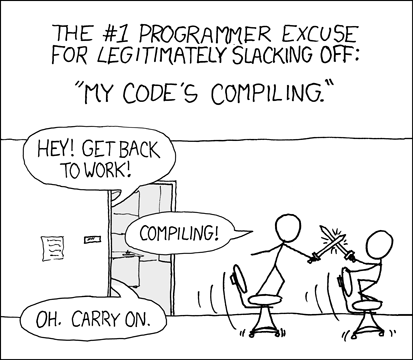
\includegraphics[width=.5\linewidth]{../compiling.png}
	\caption{%
		Compiling. \cite{xkcd/303}
	}
	\label{fig:compiling}
\end{figure}

\subsection{Umgang mit System 3}

\subsection{Versuchsaufgabe 5}

\subsubsection{Beschreiben der Funktionen}

\begin{problem}
	Beschreiben Sie die Funktionen des Programmes.
\end{problem}

Um ein Gefühl für das Programm zu bekommen, und um es schon vorher zuhause zu
testen, habe ich es in C++ nachgebaut. Dabei habe ich ausgenutzt, dass C
eigentlich nur Assembler mit Makros ist und auch über ein \texttt{goto}
verfügt. Die Ausgabe erfolgt in eine Textdatei.

\inputminted[fontsize=\small, linenos]{cpp}{../Prototypen/saegezahn.cpp}

Die \texttt{if}-Abfrage musste nur rein, damit das Programm auch terminiert.
Die Ausgabe ist wie folgt, von oben nach unten, von links nach rechts:

\begin{multicols}{9}
	\inputminted[fontsize=\footnotesize]{text}{saegezahn.txt}
\end{multicols}

Zu erkennen ist der Sägezahn, der durch den (hier gewollten) Überlauf zustande
kommt.

\paragraph{Konvertieren zu Assembly}

Um so richtig zu verstehen und zu dokumentieren, wie ich ein derartiges
Programm in 8080-Assembly übersetze, übersetze ich dieses Programm, das ich vom
Assembly abgelesen habe, wieder zurück in Assembly und dokumentiere dabei genau
die Schritte, die ich gemacht habe.

Zuerst muss die \texttt{0x00} in das Register A geschrieben werden. Dazu
benutze ich den Befehl \texttt{MVI~r}. Dieser hat einen Maschinencode von
\texttt{0b00ddd110}. Dabei ist das Ziel („Destination“, „d“) das Register A, der
Akkumulator. In der letzten Seite ist dessen Adresse mit 0b111 angegeben. Somit
setze ich meinen Befehl zusammen: \texttt{0b00111110} und noch das \texttt{0x00}.
Die erste Zahl lasse ich Python nach Hex konvertieren und erhalte
\texttt{0x3e}. Dies ist meine Zeile \texttt{0x00}.

Als nächstes kommt die Erhöhung von A. DAzu benutze ich den Befehl
\texttt{INR~r}. Dessen Maschinencode ist \texttt{0b00ddd100}, wobei ich wieder
\texttt{0b111} als Ziel einsetze. Konvertiert ist das ganze dann \texttt{0x3c}.

Jetzt folgt die Ausgabe auf den DAC-Wandler. Das Ausgabekommando ist
\texttt{OUT} und bekommt als zweites Byte das Zielregister. Dieses ist
\texttt{0x04}. Also \texttt{0xd3~0x04}.

Zuletzt kommt der Sprung zurück in Zeile \texttt{0x02}. Dazu benutze ich
\texttt{JMP}. Warum dieser Befehl zwei Bytes bekommt, und nicht nur ein Byte,
ist mir (noch) nicht klar. Das erste Byte ist jedenfalls die relevante
Zieladresse, das Zweite ist im Programm aus der Aufgabenstellung einfach
\texttt{0x00}. Dann lasse ich das auch so. Ich gehe davon aus, dass beide Bytes
die Zieladresse sind, und das ganze in Little Endian.

So sieht das fertige Programm aus:

\inputminted[fontsize=\small, linenos]{python}{../Assembly/a.s}

Es ist genau gleich mit der Aufgabenstellung, so dass die obige Erklärung
wahrscheinlich richtig ist.

\subsubsection{Ändern der Periode}

\begin{problem}
	Ändern Sie das Programm so, dass die Möglichkeit besteht, über die
	B-Register die Periodendauer variabel zu verlängern.
\end{problem}

Um die Periode zu ändern, inkrementieren wir nicht, sondern addieren einen Wert
aus Register b. Dies habe ich in folgendem, leicht modifiziertem Programm
gemacht:

\inputminted[fontsize=\small, linenos]{cpp}{../Prototypen/d.cpp}

\begin{multicols}{9}
	\inputminted[fontsize=\footnotesize]{text}{d.txt}
\end{multicols}

Dieses Programm habe ich ähnlich der Vorgehensweise aus dem vorherigen
Abschnitt übersetzt:

\inputminted[fontsize=\small, linenos]{python}{../Assembly/d.s}

\subsubsection{Anderes Signal}

\begin{problem}
	Versuchen [S]ie nun mit Hilfe des DACs ein anderes Signal, wie z.\,B. ein
	Dreieck- oder Rechtecksignal zu erzeugen. Lassen Sie dabei Ihrer Phantasie
	freien Lauf.
\end{problem}

Für ein Rechtecksignal könnte man einen Zähler verwenden, und dann die Ausgabe
umschalten, wenn dieser heruntergezählt ist. Ich möchte hier ein wenig binäre
Logik benutzen und einen überlaufenden Zähler benutzen, jedoch eine der Stellen
als Ausgabe nutzen.

\inputminted[fontsize=\small, linenos]{cpp}{../Prototypen/e.cpp}

\begin{multicols}{9}
	\inputminted[fontsize=\footnotesize]{text}{e.txt}
\end{multicols}

In Assembly:

\inputminted[fontsize=\small, linenos]{python}{../Assembly/e.s}

\subsubsection{Bit überprüfen}

\begin{problem}
	Überlegen Sie sich ein Programm, welches in der Lage ist zu erkennen, ob
	das 4.te Bit des B-Registers gesetzt ist. Ist das 4te Bit gesetzt (also
	„1“), so soll das gesamte X-Register der LED Matrix aufleuchten.
\end{problem}

Um ein Bit zu überprüfen, schaue ich mit einer Art Schablone und \txor, ob das
entsprechende Bit gesetzt ist. Mit einem Sprungbefehl, der mit 0 vergleicht,
springe ich an die entsprechende Stelle und setze meine Ausgabe entsprechend.

\inputminted[fontsize=\small, linenos]{cpp}{../Prototypen/f.cpp}

\begin{multicols}{9}
	\inputminted[fontsize=\footnotesize]{text}{f.txt}
\end{multicols}

Diese Ausgabe sind binär nur Einsen (also FF), also wurde das entsprechende Bit
gefunden. Bei FF als Eingabe war dies auch zu erwarten.

In Assembly:

\inputminted[fontsize=\small, linenos]{python}{../Assembly/f.s}
\subsubsection{Multiplikation}

\begin{problem}
	Schreiben Sie ein Programm zur Multiplikation zweiter 8-Bit-Zahlen. Der
	Multiplikand und der Multiplikator sollen an den A- und B-Registern
	eingegeben werden. Das Ergebnis (16 Bit) soll von zwei Registern der LED
	Matrix (X und R) angezeigt wwerden. Hinweis: Nutzen Sie die
	Doppelgenauigkeits-Arithmetikbefehle.
\end{problem}

Für diese Aufgabe wähle ich einen einfachen Algorithmus, und zwar:
\[
	a \cdot b = \sum_{i = 1}^{a} b
\]

Das Problem ist, dass negative Zahlen so nicht berücksichtigt werden. Ich
hoffe, dass das hier in Ordnung ist.

Dieser Rechner sieht nach Big Endian, so dass H vor L kommt. Für Intel ist das
aber eigentlich ungewöhnlich. In der C++ Version muss ich etwas basteln, um
zwei nebeneinander liegende Speicherzellen zu bekommen, die ich dann einzeln
ansprechen kann. In Assembly brauche ich das nicht, weil die Register fest
sind.

\inputminted[fontsize=\small, linenos]{cpp}{../Prototypen/g.cpp}

Die Ausgabe in den zwei Registern ist, wie erwartet (jedoch als Little Endian):

\begin{multicols}{3}
	\inputminted[fontsize=\footnotesize]{text}{g.txt}
\end{multicols}

Hier ist der Assembly-Quelltext:

\inputminted[fontsize=\small, linenos]{python}{../Assembly/g.s}

Man hätte es sich sparen können, den Zähler aus C nach A zu holen um ihn zu
dekrementieren. Jedoch hatte ich schon alle anderen Rechenschritte in A, so
dass ich dies einfach auch so gemacht habe.

Vor dem Sprungbefehl brauche ich hier keinen Vergleich, weil der
\texttt{DCR}-Befehl schon das Flag \texttt Z setzt.

%%%%%%%%%%%%%%%%%%%%%%%%%%%%%%%%%%%%%%%%%%%%%%%%%%%%%%%%%%%%%%%%%%%%%%%%%%%%%%%
%                                  Literatur                                  %
%%%%%%%%%%%%%%%%%%%%%%%%%%%%%%%%%%%%%%%%%%%%%%%%%%%%%%%%%%%%%%%%%%%%%%%%%%%%%%%

\FloatBarrier
\IfFileExists{\bibliographyfile}{
	\bibliography{\bibliographyfile}
}{}

\end{document}

% vim: spell spelllang=de tw=79
